\chapter{Gamification\label{sec:gamification}}

\section{Tecnologie persuasive\label{sec:tecnologie-persuasive}}

Una definizione di tecnologie persuasive è la seguente:
\begin{quoting}
    \omissis tecnologie interattive che mirano a cambiare il comportamento degli utenti attraverso la persuasione e l'influenza sociale senza usare inganni o forzature. \omissis
\end{quoting}

\begin{figure}[htp]
    \centering
    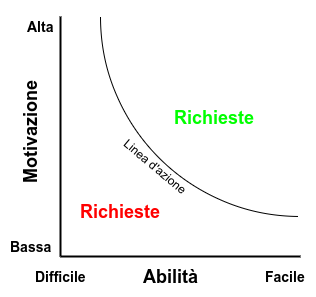
\includegraphics[width=0.5\textwidth]{immagini/Fogg_behavior_model.png}
    \caption{Fogg Behavior Model}
    \label{fig:fogg-behavior-model}
\end{figure}

B.J. Fogg ha ideato un modello per studiare il comportamento umano e come esso muta, prendendo in analisi le seguenti caratteristiche:
\begin{itemize}
    \item motivazione dell'utente per svolgere determinati compiti;
    \item abilità per assumere un comportamento (risorse che l'utente ha a disposizione, come tempo, attenzione, capacità mentale);
    \item richieste da portare a termine, che in base a motivazione e abilità possono essere più o meno efficaci nell'influenzare un comportamento.
\end{itemize}

Oinas-Kukkonen e Harjumaa hanno invece creato il Persuasive Systems Design (PSD) model, con l'obiettivo di valutare i sistemi persuasivi e di descrivere il tipo di contenuto e di funzionalità software che dovrebbero essere presenti nel prodotto finale.
In particolare PSD mette in evidenza:
\begin{itemize}
    \item Information Technology (IT) non è mai neutrale rispetto ai comportamenti delle persone;
    \item se il sistema supporta l'assunzione di impegni, gli utenti probabilmente saranno più persuasi;
    \item un individuo che valuta attentamente il contenuto del messaggio persuasivo può essere approcciato con un percorso diretto, mentre un individuo meno riflessivo e che usa semplici indizi o stereotipi può essere persuaso attraverso un percorso indiretto;
    \item la persuasione è spesso incrementale: risulta più semplice iniziare le persone a fare una serie di azioni attraverso suggerimenti incrementali, piuttosto che con un unico suggerimento fornito una tantum;
    \item contenuti basati su informazioni non fidate o false impediscono l'obiettivo finale di cambiare le attitudini o i comportamenti;
    \item i sistemi persuasivi devono mirare a non essere intrusivi e a essere semplici da usare.
\end{itemize}

Il modello PSD pone molta enfasi sul fatto che la selezione dei principi di progettazione rilevanti richiede un'attenta analisi del contesto per poter scegliere i momenti più opportuni in cui inviare i messaggi persuasivi.

Il contesto della persuasione è formato da:
\begin{description}
    \item[intento]:
    \begin{itemize}
        \item il persuasibile, ovvero determinare chi è colui che si vuole persuadere;
        \item il tipo di cambiamento, in particolare se la persuasione mira al cambiamento di un'abitudine o di un comportamento che accade una volta sola.
    \end{itemize}
    \item[evento]:
    \begin{itemize}
        \item contesto d'uso;
        \item contesto dell'utente;
        \item contesto tecnologico.
    \end{itemize}
    \item[strategia]:
    \begin{itemize}
        \item il messaggio da comunicare;
        \item il percorso da usare per raggiungere l'utente (diretto o indiretto).
    \end{itemize} 
\end{description}

Per poter essere in grado di progettare e valutare la persuasività di un sistema software bisogna comprendere sia il contenuto informativo che le funzionalità software. I principi di valutazione di sistemi persuasivi sono suddivisi in:
\begin{description}
    \item[primary task support]:
    \begin{itemize}
        \item riduzione di comportamenti complessi in semplici attività;
        \item tunneling attraverso un processo o un'esperienza che può persuadere l'utente;
        \item personalizzazione di contenuti o servizi;
        \item self-monitoring delle performance o dello status dell'utente per raggiungere obiettivi;
        \item simulazioni per far osservare il collegamento tra causa ed effetto;
        \item prove di un comportamento per cambiare le loro attitudini o comportamenti nel mondo reale.
    \end{itemize}
    \item[dialogue support]:
    \begin{itemize}
        \item elogi per favorire l'apertura alla persuasione;
        \item ricompense per il completamento di richieste;
        \item promemoria degli obiettivi da raggiungere;
        \item suggerimenti per raggiungere gli obiettivi;
        \item similarità tra utente e sistema;
        \item liking: un sistema che è visualmente attraente;
        \item ruolo sociale.
    \end{itemize}
    \item[system credibility support]:
    \begin{itemize}
        \item attendibilità;
        \item competenza;
        \item credibilità;
        \item real-world feel: un sistema che evidenzia i soggetti che ci lavorano;
        \item autorità;
        \item approvazione di terze parti;
        \item verificabilità attraverso fonti esterne.
    \end{itemize}
    \item[social support]:
    \begin{itemize}
        \item apprendimento sociale per similarità con altre persone;
        \item confronto sociale;
        \item normative influence attraverso pressione da persone simili;
        \item facilitazione sociale (altre persone mantengono il comportamento desiderato insieme a me);
        \item cooperazione;
        \item competizione;
        \item riconoscimento pubblico.
    \end{itemize} 
\end{description}

\section{Gamification e tipi di giocatore\label{sec:gamification-giocatore}}

Con il termine serious game ci si riferisce a quei giochi il cui scopo principale è educare e motivare gli utenti, attraverso la creazione di un'esperienza piacevole e accattivante. La componente ludica e di intrattenimento tipica dei giochi è quindi secondaria.
Questi tipi di giochi richiedono all'utente di mantenere la concentrazione per un lungo periodo di tempo, ovvero sono immersive.

Il termine gamification è stato definito in molti modi diversi. Viene data la seguente definizione:
\begin{quoting}
    \omissis the use of game elements and game design techniques in non-game contexts. \omissis
\end{quoting}

Un sistema con gamification non è immersive: il gioco viene svolto solo una volta ogni tanto, come gioco casuale, richiedendo quindi solo attenzione parziale da parte dell'utente.

I tipi di giocatore che sono stati identificati sono i seguenti:

\begin{description}
    \item[seekers]: giocatori a cui piace trovare qualsiasi cosa, dagli oggetti più strani e bizzarri a quelli più familiari; sono mossi dalla curiosità;
    \item[survivors]: questi giocatori amano scappare dalle minacce spaventose, adorano il rischio;
    \item[daredevils]: a questi giocatori piace superare piattaforme vertiginose, o correre ad alta velocità ma sempre mantenendo il controllo;
    \item[masterminds]: in questa categoria rientrano tutti quei giocatori a cui piace risolvere puzzle ed escogitare strategie;
    \item[conquerors]: a questa categoria di giocatori piace sconfiggere nemici difficili;
    \item[socializers]: in questa categoria rientrano tutti quei giocatori che amano andare in giro con altre persone fidate e aiutare altri giocatori;
    \item[achievers]: a questi giocatori piace collezionare qualsiasi cosa si possa collezionare.
\end{description}

Molti giochi e applicazioni utilizzano cooperazione e competizione, il supporto sociale e la pressione dei propri pari come motivatori per favorire il cambiamento di comportamento.
Nonostante meccanismi basati sui gruppi siano promettenti, studi riportano risultati conflittuali sulla loro efficacia. L'influenza sociale può infatti variare in base alle condizioni e alle caratteristiche degli individui coinvolti. È stato fatto uno studio per valutare le attitudini dei giocatori in un "health game" multiplayer e sono stati riscontrati $5$ tipi di giocatori:
\begin{description}
    \item[achievers]: si focalizzano sul miglioramento personale; a loro non piace essere sottoposti a confronti . Sono motivati dal progresso individuale e dal migliorare le proprie performance. La loro influenza su altri membri del gruppo è limitata;
    \item[active buddies]: gioiscono della compagnia di un piccolo gruppo di amici stretti che creano. Sono motivati dal "social play", si ricordano tra loro di essere attivi;
    \item[social experience seekers]: usano i mezzi di comunicazione del gioco e applicano il role-playing che questi generano come contesto dove interagire con i compagni di gioco;
    \item[team players]: i giocatori sono più motivati dai risultati di gruppo e dal ranking e incoraggiano gli altri a migliorare la performance del team; sono motivati dal senso di appartenenza e sono entusiasti di contribuire per una causa più grande;
    \item[freeloaders]: non contribuiscono al risultato di gruppo ma vi restano comunque all'interno, spesso a scapito della performance del gruppo stesso. Questi giocatori spesso perdono l'interesse velocemente, non chiedono di uscire o di essere rimpiazzati ma vi restano all'interno per vedere quale beneficio personale possono ottenere. 
\end{description}

Questa analisi ha portato alla formulazione dei seguenti principi di design e osservazioni specifici per i giochi multiplayer:
\begin{itemize}
    \item la maggior parte dell'influenza è limitata al più a un piccolo gruppo di amici;
    \item è più semplice per i giocatori coordinarsi all'interno di gruppi piccoli che hanno legami sociali oltre la competizione;
    \item visualizzare una rappresentazione online di sé in un gruppo può supportare l'attività di gruppo e creare un luogo online condiviso;
    \item alcuni giocatori mostrano interesse nel rappresentare un'immagine ideale di sé usando il loro avatar online;
    \item non è ragionevole pensare che tutti i giocatori scelgano un particolare stile di gioco e che non lo cambino mai;
    \item alcune persone possono essere particolarmente sensibili o non disposte a condividere informazioni su di sé. Occorre quindi dare ai giocatori il controllo per decidere quando condividere, quali informazioni e con chi.
\end{itemize}

\section{Gamification: utenti target\label{sec:gamification-utenti}}
Dopo aver preso in considerazione i diversi tipi di giocatore e le relative caratteristiche, abbiamo deciso in base al target di utenti identificato in precedenza di dotare il sistema delle seguenti caratteristiche:
\begin{description}
    \item[profilo]: è presente una sezione profilo personalizzabile dall'utente, ma senza troppe opzioni, in modo da restare semplice e non sovraccaricare l'utente con complessità inutile;
    \item[ranking]: c'è una classifica in modo che gli utenti possano confrontare i propri punteggi in base ai voti espressi;
    \item[privacy]: non è obbligatorio registrarsi per votare un treno. È possibile giocare senza condividere i dati relativi al proprio profilo, restando anonimi relativamente alla classifica.  
\end{description}


\section{Meccaniche di gamification\label{sec:gamification-meccaniche}}

Zichermann descrive le principali game mechanics e descrive alcune delle più importanti game dynamics che si ritrovano nelle applicazioni web e mobile più popolari.

\begin{description}
    \item[punti ricompensa]:
    \begin{itemize}
        \item punti esperienza: guidano il giocatore e gli permettono di orientarsi nell'esperienza di gioco, di capire quali sono le attività più importanti. Non si perdono mai;
        \item punti vendibili: questi punti sono guadagnati e spesi dal giocatore per ricompense esterne (regali, monete, status) o interne al sistema e sono la base per la formazione di una economia virtuale;
        \item punti abilità: sono i punti che permettono al giocatore di guadagnare ricompense per le attività svolte e sono guadagnati portando a termine azioni specifiche;
        \item punti karma: questi punti portano un guadagno al giocatore solo se condivisi;
        \item punti reputazione: misurano il livello di attendibilità di un utente e sono usati per costruire un livello di fiducia tra le parti.
    \end{itemize} 
    \item[livelli]: fungono da marcatori per i giocatori per conoscere la loro posizione nell'esperienza e nel percorso di gioco. La loro difficoltà non è solitamente lineare: si tende ad iniziare con livelli più semplici e progressivamente si va verso quelli più complessi. Solitamente un gioco viene strutturato così che il passaggio di livello avvenga dopo aver accumulato un determinato quantitativo di punti e che dia accesso a nuovi contenuti.
    \item[badge]: i badge marcano il completamento di obiettivi e il progresso nel gioco. In alcuni giochi possono anche rimpiazzare i livelli come marker del progresso. A livello di dinamiche, oltre che per mostrare uno status, le persone li desiderano per poterli collezionare, per ragioni estetiche o anche provare la piacevole e improvvisa sorpresa di averne guadagnato uno nuovo.
    \item[classifiche]: le classifiche permettono di ordinare le performance degli utenti e di fare paragoni. Ne esistono di due tipi: le "infinite leader boards", che comprendono tutti gli utenti del gioco, e le "no discentive leader boards", dove il giocatore viene posto al centro, senza badare alla sua posizione nel ranking, così che possa vedere solamente il giocatore prima e dopo di lui. La competizione risulta correlata all'aspirazione di diventare il migliore all'interno del proprio gruppo di amici.
    \item[economia di gioco]: l'adozione di determinati tipi di punti permette la costruzione di vere e proprie economie all'interno del gioco, dove l'utente non può vincere a lungo senza comprare, guadagnare e consumare determinati beni virtuali.
    \item[sfide]: le sfide corrispondono alle "missioni" che gli utenti devono compiere all'interno del gioco; danno un motivo al giocatore per continuare a partecipare al gioco, motivandoli a raggiungere risultati attraverso ricompense come trofei, badge da sbloccare. Inoltre, gli obiettivi generano confronto e competizione quando mostrati agli altri giocatori. È importante ricordare che a un giocatore novizio o ai primi livelli non vanno date sfide da livello master: è meglio dare sfide diverse per livelli diversi. Un particolare tipo di sfide sono quelle collaborative. Possono essere inserite nel gioco per creare esperienze di gruppo, dove i giocatori agiscono da soli ma i risultati vengono sommati insieme.
    \item[onboarding]: con onborading si intende l'atto di introdurre un nuovo utente nel gioco. I primi minuti in cui un utente s'impegna in un gioco sono i più importanti, perché è in questo breve lasso di tempo che prende le sue decisioni. In questi piccoli istanti non bisogna dare spiegazioni o far leggere lunghi testi con regole o istruzioni, ma bisogna fargli provare l'applicazione. Inoltre in questa fase non bisogna chiedere all'utente di registrarsi: non c'è nulla allo stato attuale che lo obblighi a fornire dati personali ad un servizio che ancora non conosce. Il processo di onborading rivela la complessità del gioco lentamente e non può fallire. Nel livello 0 (il tutorial) non ci devono essere scelte. Al giocatore vanno offerte azioni senza rischi, che non possono portare al fallimento, poi va ricompensato per aver completato l'azione con successo.
\end{description}

Altri due elementi di gamification che si ritrovano nelle applicazioni sono la personalizzazione e i feedback.
La personalizzazione può apparire in diverse forme, ad esempio, lasciando decidere all'utente come vestire il proprio avatar nel mondo virtuale; anche solo il nome del giocatore sullo schermo può essere considerato un avatar, dando quindi possibilità di personalizzazione. Tuttavia se ci sono troppe scelte di personalizzazione, la soddisfazione dell'utente cala precipitosamente.
I feedback sono le informazioni che indicano al giocatore dove si trova nell'esperienza di gioco e si vedono frequentemente nelle interazioni tra punteggi e livelli.

L'utilizzo di queste meccaniche risulta essere basilare per innescare gli activity loops, che caratterizzano i processi di gamification.
Lo scopo di questi loop è quello di nutrire l'entusiasmo degli utenti al fine di convincerli a tornare ad utilizzare il sistema. Ne esistono due tipi: engagement loop e progression loop.

Engagement loop opera a livello di azioni individuali dell'utente: quando nell'utente la motivazione è sufficientemente forte, questa porterà l'utente stesso all'azione e quindi ad utilizzare il sistema. L'azione produrrà un feedback, il quale si tradurrà in una forma di motivazione per l'utente. Così il ciclo si ripeterà.

Il progression loop considera cosa accade all'utente durante l'utilizzo del sistema nel suo insieme. Questo loop dimostra la necessità di creare degli step intermedi bilanciati così da comunicare all'utente la facilità nel raggiungerli uno dopo l'altro. All'interno del gioco, solitamente questo si traduce nell'evoluzione del giocatore (newbie - expert - master). Il primo passo consiste in on-boarding, ovvero il processo di inserimento dell'utente nel gioco nel modo più veloce ed efficace possibile. Non appena l'utente ha imparato le regole ed inizia a raggiungere i livelli più alti, sono alternati momenti di riposo, con difficoltà minore, a momenti dove la difficoltà di gioco è più alta. Mantenere sempre la difficoltà alta renderebbe il gioco troppo difficile agli occhi dell'utente, stancandolo.

Le game mechanics sono quindi essenziali per innescare questi loop. Ci sono meccaniche di gioco che funzionano bene per una determinata tipologia di giocatori e meno bene per altre. Per questo motivo è importante considerare anche le dinamiche di gioco che sono l'evoluzione temporale e i pattern sia del gioco che dei giocatori che rendono il gioco più divertente. Buone dinamiche portano il giocatore nelle fasi successive al momento giusto, così che il giocatore si senta abile ed esperto. Se non ben progettate, portano a perdere giocatori nel tempo o per noia o per il dover affrontare sfide troppo complesse, che rendono il gioco meno divertente.

\section{Meccaniche di gioco nella nostra app\label{sec:meccaniche-app}}
Per quanto riguarda la nostra app, abbiamo deciso di applicare le seguenti meccaniche di gioco:
\begin{itemize}
    \item punti esperienza e punti abilità, che permettono al giocatore di salire di livello, in modo più facile all'inizio e più difficile man mano che il gioco prosegue, ma cercando di non fornire obiettivi impossibili;
    \item badge guadagnati in base a un numero di azioni specifiche svolte;
    \item classifiche per esperienza e abilità diverse;
    \item on-boarding con tutorial: l'utente viene introdotto al gioco senza troppe spiegazioni, e in modo che riceva immediatamente una gratificazione dopo aver votato un treno. Le istruzioni vengono visualizzate per i primi tre accessi, dopodiché scompaiono e diventano raggiungibili dal menù laterale.
\end{itemize}

\section{Dinamiche di gioco e FBM\label{sec:dinamiche-fbm}}

Le dinamiche di gioco create dall'attenta combinazione delle meccaniche sono un elemento molto importante perché permettono di modificare gli elementi chiave del FBM fino ad innescare il comportamento target.
Le dinamiche offrono un modo per motivare gli utenti attraverso feedback positivi, guadagnando badge, mostrando il proprio status, ecc. Forniscono anche due approcci per aumentare l'abilità dell'utente.

Il primo consiste nel far fare pratica all'utente con l'abilità richiesta, così da aumentarla fino a superare l'activation threshold.

Il secondo, invece, si concentra nel far percepire l'abilità come semplice. Per applicare questo  approccio si possono utilizzare le seguenti strategie:
\begin{description}
    \item[divide-et-impera]: si spezza il lavoro complesso in task più piccoli e più semplici;
    \item[cognitive rehearsal]: si mostra come il lavoro è fatto e quanto è semplice;
    \item[cascading information]: istruzioni e informazioni sono rilasciate in piccoli frammenti per guidare l'utente in un task multi-fase.
\end{description}

\begin{comment}
 S OCIAL DESIGN PRINCIPLES
SOCIAL LEARNING All'interno di un contesto sociale le persone imparano l'una dall'altra, osservando i relativi comportamenti;
SOCIAL COMPARISON Quando le persone usano informazioni sugli altri per valutare se stessi, si impegnano in un paragone sociale. Questo influenza la motivazione.
N ORMATIVE INFLUENCE Questo tipo di influenza porta le persone a conformarsi allo scopo di essere piaciute ed accettate. Ciò è guidato dalla percezione della popolarità di certi comportamenti, ovvero dalle norme sociali. Gli studi dimostrano che sia le injunctive norms, che le descriptive norms sono particolarmente efficaci nell'alterare i comportamenti e le attitudini. Le prime si riferiscono alla percezione dell'individuo di quali comportamenti di altre persone sono tipicamente tenuti, le seconde alla percezione di quali comportamenti sono tipicamente approvati e disapprovati.
S OCIAL FACILITATION La presenza anche solo immaginata di persone in situazioni sociali crea un'atmosfera di valutazione, che aumenta le performance, la velocità e l'accuratezza di task ben svolti, ma riduce le performance di task meno familiari.
C OOPERAZIONE , COMPETIZIONE E RICONOSCIMENTO Questi fattori interpersonali forniscono motivazioni importanti, che non sarebbero presenti in assenza di altre persone. Le persone infatti apprezzano essere riconosciute e ciò favorisce la loro partecipazione e il loro contributo. In quanto tale, il riconoscimento motiva gli utenti a produrre più contenuti, quindi facilita anche gli sforzi cooperativi.
Questi tre principi sono particolarmente importanti, in quanto si possono ritrovare anche tra le dinamiche di gioco generate dagli elementi della gamification.
Si è infatti ampiamente parlato di come le meccaniche di punti, livelli, sfide, etc. siano utili per creare situazioni di gratificazione per l'utente. Ora ci si concentra più nel dettaglio nelle meccaniche multi giocatore, al fine di sfruttare al meglio gli elementi sociali per motivare maggiormente l'utente.
Nelle performance di gruppo occorre tenere in considerazione i seguenti principi:
•un gruppo di amici è più vicino e dà più valore ad un utente rispetto a un gruppo di sconosciuti e ciò influenza il risultato della persuasione;
• il numero di persone in un gruppo influenza il risultato della persuasione: la pressione è più forte nei gruppi più grandi, ma ciò è vero fino ad un massimo di 5 persone. Oltre questo numero, la motivazione può diminuire.
COMPETIZIONE Si ha una competizione quando più utenti cercano di raggiungere uno stesso goal che è raro o stanno cercando di guadagnare ciò che altri provano a guadagnare nello stesso  tempo.
La competizione motiva i gruppi con performance ed abilità equivalenti; senza queste premesse, la competizione demotiva. Inoltre ci sono persone che preferiscono competere con se stesse più che con altri.
I premi per i vincitori devono avere importanza relativa, in quanto gli sforzi del giocatore devono essere intrinseci e non guidati dal risultato atteso. Inoltre, la competizione dev'essere lunga abbastanza da evitare che i nuovi partecipanti si demotivino a causa di risultati iniziali non buoni e assicurare che tutti i partecipanti abbiano buone opportunità di vincere fino alla fine dell'attività.
Lo scopo di una competizione va fatto emergere nell'intero processo e non nei risultati.
COOPERAZIONE Con la cooperazione gli utenti interagiscono per raggiungere gli stessi obiettivi lavorando insieme. Il combinare i punteggi e risultati di più persone può incoraggiare gli utenti a cooperare.
La cooperazione porta benefici sociali, quali socializzazione e divertimento di gruppo. In determinate circostanze, può inoltre essere un maggiore elemento di motivazione rispetto
alla competizione.

M ASS I NTERPERSONAL P ERSUASION (MPI)
Nell'ambito della socialità e della tecnologia è divenuto inevitabile interrogarsi sull'utilità dei social network allo scopo di persuadere. B.J. Fogg conia il termine Mass Interpersonal Persuasion, con il quale intende il fenomeno che unisce il potere della persuasione interpersonale con la portata dei mass media grazie all'avvento dei social network.
La MPI comprende 6 componenti:
• Persuasive Experience: è l'esperienza creata per cambiare attitudini o comportamenti.
•Automated Structure: la tecnologia digitale automatizza l'esperienza persuasiva e la rende ripetibile, permettendo agli utenti di condividerla con altri in modi più semplici.
•Social Distribution: social network sono importanti per MIP perché rendono l'esperienza persuasiva più credibile e la distribuzione più semplice di quanto succede nell'Internet aperto. L'esperienza persuasiva è condivisa da un amico all'altro. Un amico può invitarne un altro ad unirsi all'esperienza. Il processo si ripete con i nuovi amici che coinvolgono i loro amici.
Inoltre, l'esperienza persuasiva guadagna credibilità dall'essere all'interno delle mura protettive del social network.
•Rapid Cycle: l'esperienza persuasiva può essere distribuita velocemente da una persona all'altra.
•Huge Social Graph: l'esperienza persuasiva può potenzialmente raggiungere milioni di persone connesse attraverso legami e/o interazioni sociali;
•Measured Impact: l'effetto dell'esperienza persuasiva è osservabile dagli utenti e dai creatori; ad esempio facebook platforms mette a disposizione sia dei creatori che a coloro che usano l'app di vedere le statistiche base sulla distribuzione ed uso dell'applicazione.
\end{comment}